\section{Project Description}
The ''Portfolio Management Game'' was initially developed in 2001 by an external company for the Department of Banking and Finance at the University of Zurich. This simulation of a portfolio manager was being used from the DBF over several years by multiple seminars of their departement. A course named ''Advanced Portfolio Seminar'' has given insights to the portfolio management process for Master students by playing the game in between different rounds playing the game. For the final seminar of the ''Executive Education'' the game was being played for two days on Uetliberg with all the executive students.\\

The game has been deprecated by its implemented technologies and after each round the supervisors had to collect a USB-stick where all decisions of the students have been saved to. The supervisors had to collect this data for each group on a central device with administrative access (on a windows native application) to calculate the result of the teams decisions.

\begin{center}
  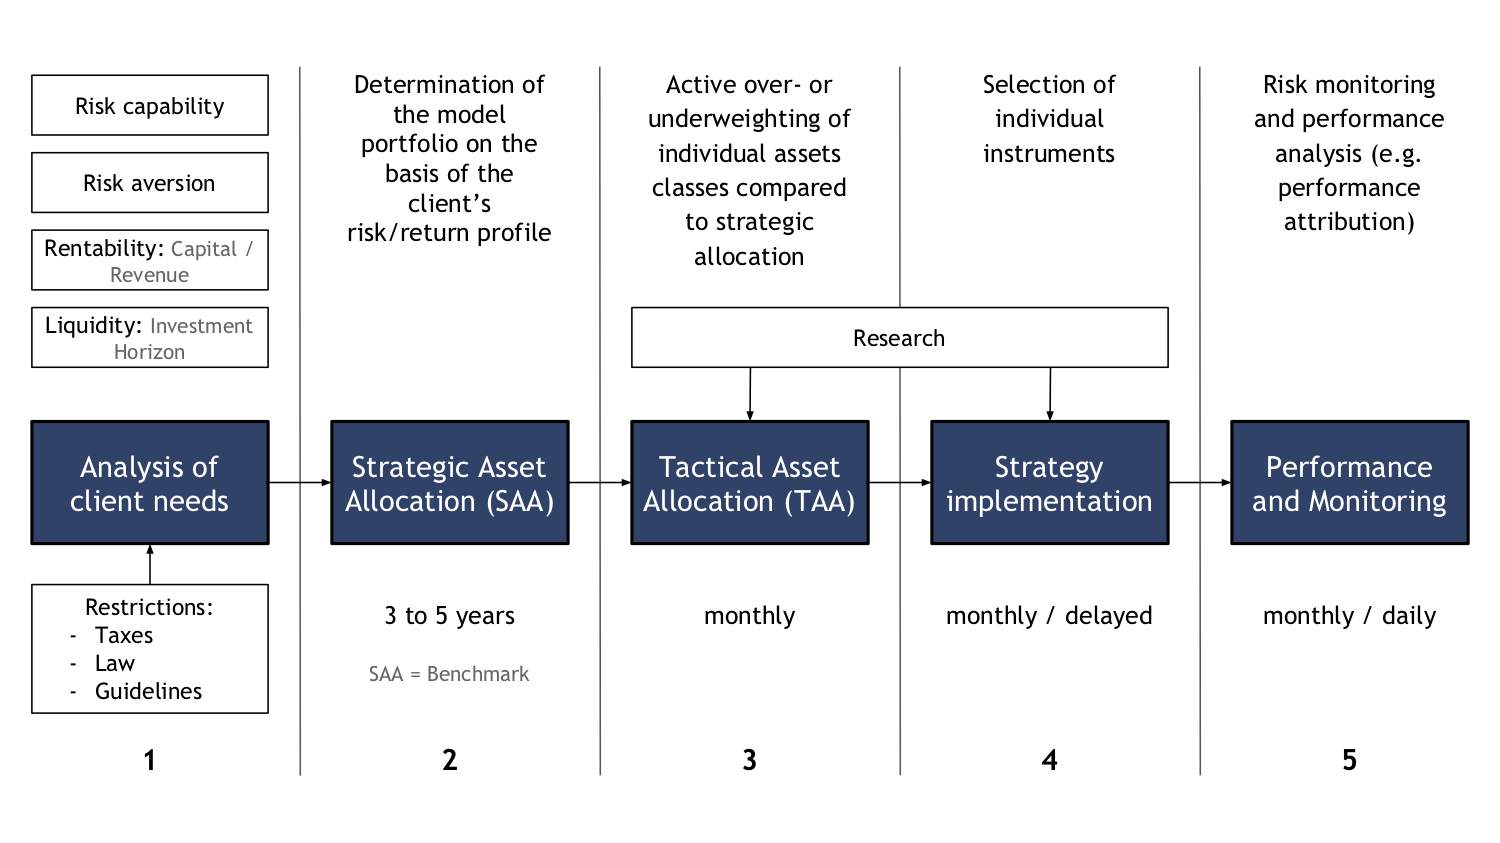
\includegraphics[scale=0.5]{img/private_banking_process.png}
\end{center}
